\section{Optimizations}
\label{optimization}
%- Motivation für Optimierungen
%	- Ungenutze Slices
% 	- Vollständige Auslastung der belegten Komponenten

If one were to implement a Bitcoin Mining FPGA as described earlier, though functional, it would be highly inefficient both in terms of speed and utilization of the logic slices available, approximately computing one Bitcoin double hash every 192 cycles\footnote{The initial header is 640 bits long, padded to 1024 bits. The first stage of the Bitcoin double SHA-256 takes two iterations, one for each 512-bit chunk. Of these two iterations, each takes 64 rounds for extending the chunks into the message array and applying the compression function, adding up to $2 \cdot 64$ = $128$ cycles (if one round is calculated in one cycle). The second stage of the Bitcoin double SHA-256 receives the result of the first one, a 256-bit message, which is then padded to 512 bits. This leads to one iteration, meaning $64$ rounds of the extender and compressor. Summing these values up, a total of $128+64$ = $192$ cycles is needed per Bitcoin double hash, without accounting for the time needed for padding and synchronization of the components.}, if optimally implemented. In the following three subsections we aim to give more insights into the optimizations used to increase the rate at which the FPGA computes the Bitcoin double SHA-256 and methods used to more efficiently employ the logic slices available to us. The first subsection details the way our implementation handles parallelization, the second describes the usage of pipelining in this use case, and the final section catalogs the optimizations we applied to the individual components.


\subsection{Parallelization}

%- Motivation -> Mehr Ressourcennutzung
The first optimization analyzed will be parallelization, where the main motivation is to more effectively utilize the resources available to us.

\subsubsection{Mining Core Component}
\label{mc_component}

%- Erzeugung der Mining-Cores
%   - Mining-Core als multiplizierbare Komponente

In order to parallelize our system, we implemented the here-called mining core. This component needs to fulfill three demands in order to be useful for our parallelization efforts:

\begin{enumerate}
	\item Compute hashes for a fixed set of nonces.
	\item Evaluate whether it has found a valid nonce.
	\item Be resettable.
\end{enumerate}

To realize these, this component is given a certain nonce generation scheme, threshold, and header with which it continuously computes SHA-256d hashes. It does this by appending the current nonce generated through the externally provided algorithm to the header for which a valid hash is desired, computing a hash, and repeatedly regenerating the next nonce through the previously named scheme until a hash satisfying the given threshold is found.
This functionality is executed by extending our previous SHA-256 implementation through prepending a nonce generator and appending a comparator component. The nonce generator computes the next nonce with which the header is to be padded according to the given technique and the comparator verifies if the computed hash matches the provided constraints, setting an output signal in the case where it does.
Finally, the mining core is resettable through an input signal that can be set by an external actor, which is asynchronously redirected to all subcomponents of the mining core, thereby interrupting all computation inside of it and reseting all subcomponents to their initial state. Through these three extensions, we have now created a controllable, multipliable unit capable of computing SHA-256d.


\subsubsection{Distribution of Work}
%   (Nonces)
% 	- Wie verteilen wir?
% 	- Warum werden damit alle Nonces abgedeckt?
%	- Was ist die beste Start-Nonce?

The next aspect to realizing this parallel system is to define the above named nonce-generation algorithm that is to be used for assigning groups of nonces to a mining core. Due to the only aspect of a given nonce being influential on the time of computation being its length (which is constant across nonces) and SHA-256's preimage resistance all nonces are equally valuable. 
Since no nonce leads to a faster computation or greater chance of success, the only demand our algorithm has to meet is to avoid duplicate computations using the same nonce. 

To achieve this, we define the following algorithm:

\begin{enumerate}
	\item Given \(n\) mining cores \( \{c_0, ... , c_{n-1}\} \), compute its modulo remainders \( \{0, ... , n-1\} \).
	\item Assign each mining core $c_i$ their corresponding modulo remainder $i$.
	\item A mining core computes their first hash using $i$ as a nonce. If this hash is not valid, it keeps generating nonces and hashing with them by continuously adding $n$ to their $i$.
\end{enumerate}

Since each natural number $a$ (and the nonce can be interpreted as a natural number at no penalty in this case) can be written as \( a = i + b \cdot n \) where $i$ is a modulo remainder of $n$ and $b$ is some natural number, this algorithm ensures all possible nonces are hashed. Additionally, since this expression is unique for each nonce (as each nonce can only have one modulo remainder) the algorithm also ensures no two mining cores compute using the same nonce.


\subsubsection{Mining Core Synchronization}

%- Wie fassen wir die Ergebnisse der Cores zusammen? (Nonce Master, Bus-Protokoll)

Finally, we need to deduce a methodology to reduce all results we get from each mining core while keeping performance penalization to a minimum. To do this, we create a corrsponding multiplexer component for each mining core, as shown in figure \ref{fig:multiplexer}.
where the last multiplexer points to the receiver of the reduced information, in our case a component that communicates this information to an external actor, as described in Section \ref{ssec:externalCommunication}. 

\begin{figure}
	\centering
	\includegraphics[width=\textwidth]{img/multiplexer.png}
	\caption[Architecture of our system including multiplexer for result reduction]{Architecture of our system including multiplexer for result reduction}
	\label{fig:multiplexer}
\end{figure}

The setup above yields a few advantages: 

First, due to its simplicity, it can be implemented on hardware using just a few logic gates, making it rather small. This is relevant, as keeping this component small allows for more space to place mining cores which increase performance.

Next, evaluating this chain of multiplexers does not require waiting on the presence of any signals and can therefore be evaluated fully concurrently, meaning the impact on performance is absolutely minimal. The reason there is no need to wait on the presence of any signals is due to the design of the mining core: The found signal outgoing from each core is set to 0 by default, however, the nonce signal is set as soon as the next nonce is generated by the nonce generator. This premature setting of the nonce is not an issue, as the chain of multiplexers filters out nonce signals whose corresponding found signals are not set. The advantage of the just-described configuration is that this way in the case where we find a valid nonce, by the time the found signal is set, the nonce signal will already have been defined for the whole duration of the SHA-256d hash computation. This ensures we avoid the case where a valid found signal is sent prior to the updated nonce arriving.

An additional property of this structure is the way it handles the (extremely unlikely) case that two cores both compute a valid hash at the same time using two different nonces. As can be seen from figure \ref{fig:multiplexer}, this case is handled by selecting the nonce from the core with the greater index, which in this case serves no direct purpose. The reason we can do this, is due to the fact that the value of a nonce is entirely irrelevant to the Bitcoin Network, as long as its hash concatenated behind its header is lower than the mining target at the time of its mining.

\subsection{Pipelining}

In general, pipelining does not reduce the duration of computation but it improves the throughput, allowing for greater utilization of the logic cells. The computation is divided into stages so that the hardware of each stage can process different inputs with the stages working concurrently. To ensure the optimal throughput, each stage has to take the same amount of time, else the throughput will be defined by the slowest stage, as others must wait for it to complete. Additionally, the pipeline has to be ‘filled’ to function the best, which means that n computations have to be ongoing for n stages. This concept is illustrated in figure \ref{fig:pipelining}. In our case, as resets happen infrequently, the pipeline will almost always be filled.

\begin{figure}
	\centering
	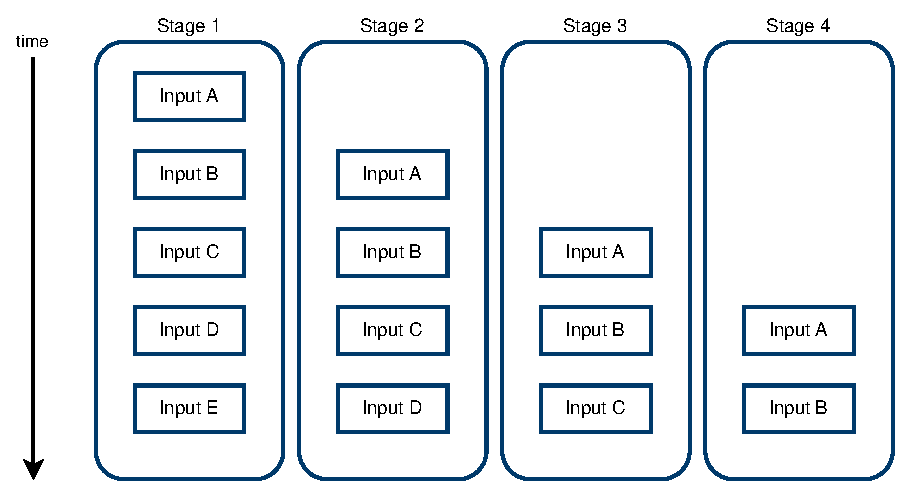
\includegraphics[width=\textwidth]{img/Pipelining.eps}
	\caption[Filling of a pipeline]{Filling of a pipeline}
	\label{fig:pipelining}
\end{figure}

%- Motivation -> Bessere Ressourcenauslastung
%- Warum haben wir die Pipeline nicht komplett ausgerollt?
%   - Großer Platzverbrauch von 64 Extendern + Compressoren

\subsubsection{Simple Pipelining}
\label{pipelining}

For the mining core, the division into stages is apparent: the first and the second SHA computations become the two stages of the pipeline. Without this pipelining, the first set of components previously had to wait for the second hash to complete before beginning to process the next block header. Now, after the first hash is computed, it is cached in a buffer between the stages, meaning the first stage can proceed to process the next block header, while the second stage works with the cached hash of the current block header, as seen in figure \ref{fig:mining-core-pipeline}.

\begin{figure}
	\centering
	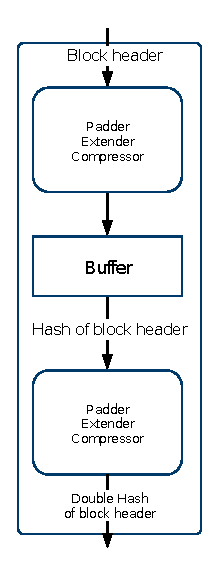
\includegraphics[width=5cm, height=9cm, keepaspectratio]{img/Mining-core-pipeline.eps}
	\caption[Pipelined mining core]{Pipelined mining core}
	\label{fig:mining-core-pipeline}
\end{figure}

Upon closer examination, we determine the durations of the stages: stage 1 takes $2 \cdot 64$ compression rounds, while stage 2 takes only 64 rounds. So, with the pipeline filled, the throughput is $1$ block header / $2 \cdot 64$ rounds, compared to $1$ / $3 \cdot 64$ rounds without pipelining.

%- Buffer zwischen den beiden SHA-256 Stufen
%- Entsprechende Abstimmung der Stufen

\subsubsection{Use of Length Extension Vulnerability of SHA-256}
\label{length_extension}

Upon closer inspection, however, we can do even better: In the first stage of SHA-256d, we want to compute \textbf{SHA-256}(\textit{header}), which we achieve by running the extension and compression function over the first 512 bits of the header, saving this state for the compression function, padding the remaining 128 bits of the header, and running the extension and compression function over these. Notice, however, how the first 512 bits contain the version of the block, the previous block hash, and part of the merkle root hash. All are values that remain constant between different mining cores and over time for a given header, as the only values that are changed are the nonce and the timestamp, both of which are contained in the last 128 bits.

We can take advantage of this by slightly changing the structure and functionality of our mining core: We designate a single mining core with an additional out-port that outputs a 256-bit vector which is then fed into the other mining cores. The content of this buffer will be the hash of the first 512 bits of the block header. Due to the length extension attack vulnerability SHA-256 \footnote{ If given \textbf{Hash}(\textit{$m_1$}) and the length of $m_1$, an attacker can compute \textbf{Hash}(\textit{$m_1$ | $m_2$}) where $m_2$ is some message controlled by the attacker, the hashing algorithm is vulnerable to length-extension attacks. SHA-256 is a special case, as an attacker can compute \textbf{Hash}(\textit{$m_1$ | $m_2$}) using only \textbf{Hash}(\textit{$m_1$}) without knowing the length of $m_1$. The reason for this is that  \textbf{Hash}(\textit{$m_1$}) is the state of the compression function after running over the final chunk of $m_1$. If $m_a$ were defined as $m_1$ | $m_2$, the hash for $m_a$ could be computed by taking \textbf{Hash}(\textit{$m_1$}) as the state for the compression function and running the compression and extension function over the added chunks from $m_2$. To be clear, an attacker did not need to know the value of $m_1$ in the previous example to compute \textbf{Hash}(\textit{$m_a$}), knowing \textbf{Hash}(\textit{$m_1$}) was sufficient. In our case, $m_a$ can be viewed as the header, $m_1$ as its first 512 bits, and $m_2$ as its last 128 bits respectively. }
 has, we can feed this resulting hash into the initial state of each compressor of the other mining cores and thereby skip computing the hash of the first 512 bits of our header for the remainder of the time we mine using it. Although this solution has the downside that for the time needed to compute the hash of the first 512 bits of the block header all but one mining core are not working, the upside in comparison is huge: For each nonce we compute SHA-256d for, we skip the amount of time we waited at the beginning for the designated mining core to compute the hash of the first 512 bits.

One may ask themselves why we opted for having one mining core compute this initial hash and distribute it to the others instead of having each core compute the initial hash themselves (which would come at no speed penalty, as this computation would be running on each core in parallel and with no time difference between cores). While the just-named solution provides the advantage of eliminating the communication overhead between cores, it requires an additional 256-bit buffer in which each mining core would need to store this hash. \newline
In our implementation with the hash distribution, the compiler of the VHDL code appears to be smart enough to realize that all mining cores are reading out the same hash and therefore can optimize the space needed for this by presumably reusing the route connecting the computed hash to each mining core. In the case of having each mining core compute the hash for themselves, the compiler does not have as much opportunity for optimization. Therefore, though in most cases our implementation is likely more space-optimal, the choice for which design-choice of said length-extension attack is ultimately compiler-specific. 


%- Motivation -> Vermeidung von Doppelberechnungen, Bessere Ressourcenauslastung (Nicht mehr 2 auf 1)
%- Warum geht das mit SHA-256? Warum geht das bei Bitcoin?
%- Kurze Erklärung von length extension attack

%- Erklärung der Speicherung
%- Wo speichern wir?
%- Verteilung an andere Mining Cores
%- Warum macht es Sinn nur einen rechnen zu lassen und nicht alle? (-> Buffer nur 1x)
%- Sind die 64 Cycle am Anfang die nur ein Core rechnet hinnehmbar?

\subsubsection{Compressor pipelining}

Another interesting optimization idea is to further roll out the pipeline for each of the two hashing stages. For this, both stages would be split into 64 sub-stages, each of which correspond to one round of the SHA-256 algorithm. As a result, each mining core would only contain one nonce generator, padder and comparator, but $2 \cdot 64$ extenders and $2 \cdot 64$ compressors.

The main reason speaking against this optimization is that there aren't enough logic cells on the target FPGA board. This becomes clear by estimating the maximum saved area compared to our final implementation. As the two extender and two compressor components jointly take up around 85\% of a mining core's logic cells, completely rolling out the pipeline while not changing the hash components themselves would increase the size of a single core $ 0,85 \cdot 63 + 1 \approx 55$ times. However, the constants of the compressor $K$ and the compressor buffer, described in section \ref{length_extension}, are only needed once per core and could be optimized in a rolled out pipeline. Removing them would decrease the size of a mining core by approximately 10\%, still making it $ 0,9 \cdot 0,85 \cdot 63 + 1 \approx 49$ times larger than our final implementation. Given that our final implementation includes 16 cores, a single "rolled-out" core, which is 49 times larger, doesn't fit on the target board.


%- ausgerollter, concurrent compressor


%- moved to Timing
%-4 iter - slack, und zu gross; langsamere clock hilft nicht
%-2 iter - bonus, extender parallel

\subsection{Optimization of Single Components}

Aside from parallelization and pipelining, we applied hardware-specific timing and area optimizations to single components to do more work in one cycle and to allow for more mining cores to be deployed on the FPGA board.

\subsubsection{Timing}
\label{timing}

In FPGA design, timing closure is a vital task and can be achieved by reducing the length of critical paths. As for our mining cores, using only the rising clock edge and transferring as few data outside of the mining core entities as possible solved most timing issues at first. The longest critical path after timing optimizations, however, is located in the compressor component, making it the main limitation for a mining core's throughput. In our final implementation, the compressor already caused some timing violations with a 100 MHz clock, but our deployment tests showed that these violations weren't significant enough to influence the correctness of the calculated hashes. Yet, we weren’t able to raise the clock frequency to 200 MHz because of these timing violations.

\subsubsection*{Compressor Unrolling}

To increase the amount of work done per clock cycle, we attempted to perform multiple compressor rounds in a single cycle.

\begin{figure}
	\centering
	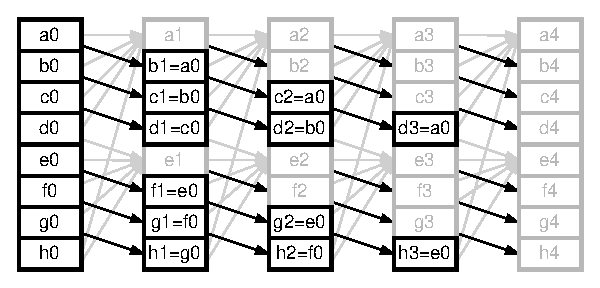
\includegraphics[width=\textwidth]{img/Compressor-dep.eps}
	\caption[Permutation of state words in four compression rounds]{Permutation of state words in four compression rounds}
	\label{fig:compressor-dep}
\end{figure}

Due to the structure of the internal state transformations, as depicted in figure \ref{fig:compressor-dep}, four rounds per cycle is the most straightforward unrolling of the compressor. Sadly, this version introduces a much longer critical path than is possible within a clock cycle. Additionally, the massive size increase of the components through this optimization means less cores fit on the FPGA board and therefore removes the possibility of managing the increased critical path by lowering the clock frequency, as this would impact performance more than the original optimization improves it. Due to these reasons, we didn't pursue this variant any further.

With an unrolling factor of two (rounds per cycle), a single mining core runs without timing issues on our standard clock speed. This is in part due to the two message digest words being able to be computed concurrently in the extender (as there are no data dependencies between them). Additionally, the total size increase of a mining core is smaller than two, which means that we would observe a net gain in performance for 12 or more functional cores (compared to 23 non-unrolled cores). We found the most problematic critical path to be during the cycle when the mining cores first receive the buffered hash of the first chunk of a header. Already for 14 cores, these critical paths are too long for our clock speed and cause the calculations to fail. While 13 cores would already increase our performance, 17 was our target, bounded by the number of logic cells available. To reach that goal, we reverted our changes to the shared buffer in hopes of reducing the critical path by buffering the first header hash inside each mining core. While this change did increase the size of the components, we could get 16 cores to run without timing issues.

%- We sadly could not arrive at 17 cores, but we speculate that introducing a stall cycle to break up the critical path would be a possibility. -> Verworfen, da durch stall cycle mining core zu groß wurde



\subsubsection{Area}
\label{size}
%- Register(Arrays) minimieren
%- Schmalere Kommunikationskanäle
%- Concurrent statt Process
%- Hardcoden von Padder
%- Entities Mergen hat nicht unbedingt starken Einfluss auf Größe, z.B. Generator & Padder
%- Verschiedene Versionen des Padders

%- TODO compressor optimizations https://gitlab.lrz.de/lrr-tum/students/eragp-blockchain-2020/-/commit/ca71addf94ee2fcdc328cf6099083acd89c685f1

By decreasing the size of each mining core, more mining cores can fit on the FPGA board, and consequently the overall performance increases. In this chapter, we will take a look at different techniques to optimize the area occupancy of our Bitcoin mining implementation. It is important to notice beforehand, that the logic cells of the VHDL entities are sometimes counted towards different components by the Vivado synthesis. Thus, the total number of logic cells belonging to a mining core is a more reliable measurement than those of a single component. In the following, all quantified logic cell optimizations of a component will assume that the other components didn't change in size unless noted otherwise.

First of all, some components of our implementation contained buffers, which could be removed without affecting the correctness of the Bitcoin mining algorithm. For example, the padder between the compressor of the first SHA-256 stage and the extender of the second stage doesn't need an internal 256-bit vector to store the intermediate hash as the compressor's output hash isn't changed before the next hash is calculated. Removing the redundant buffer from the padder reduced its size from 354 cells to 2 cells. Analogously, the internal comparator buffer could be removed by directly using the output of the second compressor. This decreased the comparator size from about 260 cells to just 7 cells.

Another method to reduce the number of logic cells per mining core is to lower the number of bits transferred between components. As an example, a mining core  only transmits the found nonce (32 bits) to the main entity instead of the calculated hash digest (256 bits) or the whole block header (640 bits).

\subsubsection*{Extender Size Optimization}
Out of all component size optimizations, reducing the extender size resulted in the most significant area enhancement as the two extenders initially were the largest components within each mining core. The vast majority of logic cells occupied by the extender was used by the 64-entry message schedule array.

In section \ref{sha256} we already learned that the first step of the SHA-256 hash computation is to prepare the message schedule using the 16 padded message blocks. This task is assigned to the extender component in our implementation. Using formula \ref{eq:extender}, it can be seen that the first 16 values of the message schedule are directly copied from the padded chunk, and calculating $W_t$ for $16 \leq t \leq 63$ only depends on the 2nd, 7th, 15th and 16th preceded message schedule array entries as demonstrated in figure \ref{fig:extender-dep}. Since previous message schedule entries are exclusively used within the extender and only the most recent value is important for the compressor calculations at a time, it is possible to reduce the message schedule size from 64 to 16 entries by accessing all indices modulo 16. Algorithm \ref{Algo:Extender1} implements this idea.

\begin{figure}
    \centering
    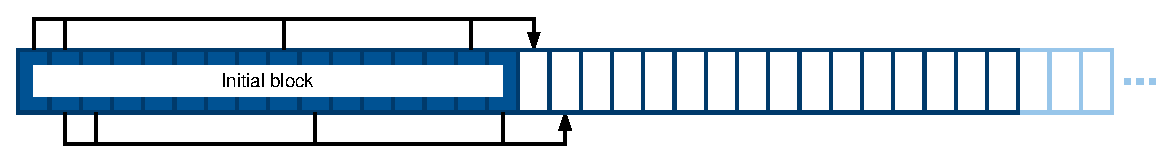
\includegraphics[width=\textwidth]{img/Extender-dep.eps}
    \caption[Data dependencies of extender]{Data dependencies of extender}
    \label{fig:extender-dep}
\end{figure}

\begin{algorithm}[H]
\caption{Pseudocode of the simplified extender with a 16-entry message schedule array}
\label{Algo:Extender1}
\begin{algorithmic}[1]
\Require{functions $\sigma_0$, $\sigma_1$ and padded chunk $M[0 \dots 15]$} 
    \State ARRAY $W[0 \dots 15]$
    \For{$t \gets 0$ to $63$}
        \If{$t < 16$}
            \State{$W[t] = M[t]$}
        \Else
            \State {$W[t \mod 16] = \sigma_1(W[(t-2) \mod 16])+W[(t-7) \mod 16] + \sigma_0(W[(t-15) \mod 16])+W[t \mod 16]$}
        \EndIf
        \State \Call{Send\_Next\_Word\_To\_Compressor}{$W[t \mod 16]$}
    \EndFor
\end{algorithmic}
\end{algorithm}

The FPGA hash rate can be further improved by swapping out the extender array into the block RAM or - if available on the FPGA board - into the distributed RAM. The block RAM typically consists of dedicated SRAM cells on the FPGA board, whereas the distributed RAM is generated with the logic cells' lookup tables. Block RAMs are generally well suited for large memories that does not occupy any logic cells. Distributed RAMs, in contrast, are ideal for smaller memories and need significantly fewer logic cells to store data compared to flip flops. For both memory types, the write operation is synchronous. The read operation on distributed RAMs is asynchronous, unlike the synchronous read on block RAMs.

The use of a RAM type can either be instantiated manually by the HDL programmer or automatically by tools such as the Vivado synthesis tool. We opted to let Vivado choose the best RAM type for the extender array, as suggested by the Vivado synthesis documentation \cite{VivadoSynthesis}. This keeps the VHDL source code flexible and portable. To let the extender array be automatically memory-optimized by Vivado, we had to remove the assignment during an asynchronous reset to make sure writing into the array only takes place synchronously. Through using the distributed RAM, the extender size decreased from around 1500 logic cells to just 300 logic cells.
% - LINK: https://www.xilinx.com/support/documentation/sw_manuals/xilinx2016_4/ug901-vivado-synthesis.pdf; page 99

Employing the distributed RAM for the extender with two rounds per cycle is a bit more complex because depending on the exact FPGA board, the distributed RAM might only have a single write port, but two entries need to be stored per clock cycle.
To fix this problem, we decided to split the internal 16-entry extender array into two 8-entry arrays, one for the former even indices and the other one for the odd indices. Algorithm \ref{Algo:Extender2} specifies this approach in greater detail. As a result, the extender size dropped from 2100 logic cells to 1000 logic cells.

\begin{algorithm}[H]
\caption{Pseudocode of the extender with two rounds per cycle and two 8-entry message schedule arrays}
\label{Algo:Extender2}
\begin{algorithmic}[1]
\Require{functions $\sigma_0$, $\sigma_1$ and padded chunk $M[0 \dots 15]$} 
    \State ARRAY $W_A[0 \dots 7]$
    \State ARRAY $W_B[0 \dots 7]$
    \For{$t \gets 0$ to $31$}
        \If{$t < 8$}
            \State{$W_A[t] = M[2*t]$}
            \State{$W_B[t] = M[2*t+1]$}
        \Else
            \State {$W_A[t \mod 8] = \sigma_1(W_A[(t-1) \mod 8])+W_B[(t-4) \mod 8] + \sigma_0(W_B[t \mod 8])+W_A[t \mod 8]$}
            \State {$W_B[t \mod 8] = \sigma_1(W_B[(t-1) \mod 8])+W_A[(t-3) \mod 8] + \sigma_0(W_A[(t-7) \mod 8])+W_B[t \mod 8]$}
        \EndIf
        \State \Call{Send\_Next\_Words\_To\_Compressor}{$W_A[t \mod 8], W_B[t \mod 8]$}
    \EndFor
\end{algorithmic}
\end{algorithm}

%- distributed RAM explanation: https://www.xilinx.com/support/documentation/application_notes/xapp464.pdf
